% ============================================================
% DATA MINING PROJECT REPORT TEMPLATE
% Department of Computer Science
% University of Pisa
% ============================================================
%
% Recommended compiler: pdflatex
% ============================================================

\documentclass[a4paper,11pt]{article}

% ============================================================
% 1. GENERAL CONFIGURATION
% ============================================================

% ------------------------------------------------------------
% FONT
% ------------------------------------------------------------
\usepackage[T1]{fontenc}
\usepackage[utf8]{inputenc}

% Main font
\usepackage{newtxtext}

% ------------------------------------------------------------
% LINE SPACING
% ------------------------------------------------------------
% DO NOT MODIFY
\usepackage{setspace}

% Examples:
% \singlespacing
% \onehalfspacing
% \doublespacing

\setstretch{1}

% ------------------------------------------------------------
% PAGE MARGINS
% ------------------------------------------------------------
% DO NOT MODIFY
\usepackage[
    top=2.5cm,
    bottom=2.5cm,
    left=2.7cm,
    right=2.7cm
]{geometry}

% ============================================================
% 2. PROJECT INFORMATION
% ============================================================

\newcommand{\CourseName}{Data Mining}
\newcommand{\DepartmentName}{Department of Computer Science}
\newcommand{\UniversityName}{University of Pisa}

\newcommand{\AcademicYear}{2026/2027}

\newcommand{\ProjectTitle}{Information Operations on Social Media}

% Add the projectID here
\newcommand{\GroupID}{Group XX}

% ------------------------------------------------------------
% LOGOS
% ------------------------------------------------------------
\newcommand{\UniversityLogo}{images/unipi_logo.png}
\newcommand{\ProjectLogo}{images/project_logo.png}


% ============================================================
% 3. PACKAGES
% ============================================================

\usepackage{graphicx}
\usepackage{booktabs}
\usepackage{array}
\usepackage{tabularx}
\usepackage{multirow}

% Subfigures
\usepackage{subcaption}

% Mathematics
\usepackage{amsmath}
\usepackage{amssymb}

% Better lists
\usepackage{enumitem}

% Colors
\usepackage{xcolor}

% URLs
\usepackage{xurl}

% Hyperlinks
\usepackage[
    colorlinks=true,
    linkcolor=black,
    citecolor=black,
    urlcolor=blue
]{hyperref}

% Headers and footers
\usepackage{fancyhdr}

% ============================================================
% 4. SECTION / TABLE OF CONTENTS DEPTH
% ============================================================

% Include:
%   sections
%   subsections
%   subsubsections
%
% in both numbering and Table of Contents.

\setcounter{secnumdepth}{3}
\setcounter{tocdepth}{3}


% ============================================================
% 5. REFERENCES
% ============================================================
\usepackage[
    backend=biber,
    style=numeric,
    sorting=nyt,
    giveninits=true,
    maxbibnames=99
]{biblatex}

\addbibresource{references.bib}


% ============================================================
% 6. PAGE STYLE FOR THE REPORT BODY
% ============================================================

\pagestyle{fancy}
\fancyhf{}

% Page number centered in footer
\fancyfoot[C]{\thepage}

\renewcommand{\headrulewidth}{0pt}
\renewcommand{\footrulewidth}{0pt}


% ============================================================
% DOCUMENT
% ============================================================

\begin{document}


% ============================================================
% TITLE PAGE
% ============================================================

\begin{titlepage}

\thispagestyle{empty}

\begin{center}

% ------------------------------------------------------------
% LOGOS
% ------------------------------------------------------------

\begin{minipage}[c]{0.45\textwidth}
    \centering
    \includegraphics[height=4.5cm]{\UniversityLogo}
\end{minipage}

\vspace{1.5cm}

{\Large \UniversityName}

\vspace{0.2cm}

{\large \DepartmentName}

\vspace{1.8cm}

{\Large \textbf{\CourseName}}

\vspace{0.5cm}

{\large Project Report}

\vspace{1.5cm}

{\huge \textbf{\ProjectTitle}}

\vspace{0.5cm}

\begin{minipage}[c]{0.45\textwidth}
    \centering
    \includegraphics[height=3cm]{\ProjectLogo}
\end{minipage}


\vspace{1.5cm}

{\Large \textbf{\GroupID}}

\vspace{0.5cm}


% ------------------------------------------------------------
% STUDENTS
% ------------------------------------------------------------

{\Large % MAKE THIS SMALLER IF YOUR DATA DOES NOT FIT
\begin{tabular}{llll}

StudentName1 & StudentSurname1 & StudentId1 & StudentEmail1 \\

StudentName2 & StudentSurname2 & StudentId2 & StudentEmail2 \\

StudentName3 & StudentSurname3 & StudentId3 & StudentEmail3 \\

\end{tabular}
}


\vfill

{\large Academic Year \AcademicYear}

\end{center}

\end{titlepage}


% ============================================================
% FRONT MATTER
% ============================================================
%
% No page numbers are displayed in:
%
% - Table of Contents
% - List of Figures
% - List of Tables
%
% These pages therefore DO NOT count toward the report limit.
%

\clearpage

\pagenumbering{gobble}


% ------------------------------------------------------------
% TABLE OF CONTENTS
% ------------------------------------------------------------

\tableofcontents


% ------------------------------------------------------------
% LIST OF FIGURES
% ------------------------------------------------------------

\clearpage
\listoffigures


% ------------------------------------------------------------
% LIST OF TABLES
% ------------------------------------------------------------

\clearpage
\listoftables


% ============================================================
% START OF THE ACTUAL REPORT
% ============================================================
%
% IMPORTANT:
%
% Page numbering starts from 1 HERE.
%
% Therefore:
%
% Title page             -> not counted
% Table of Contents      -> not counted
% List of Figures        -> not counted
% List of Tables         -> not counted
%
% The first report page  -> Page 1
%
% ============================================================

\clearpage
\pagenumbering{arabic}
\setcounter{page}{1}

\pagestyle{fancy}


% ============================================================
% 1. INTRODUCTION
% ============================================================
% ============================================================
% EXAMPLE REPORT CONTENT
% ============================================================
% ============================================================

\section{Introduction}

Euler's identity is one of the most celebrated equations in
mathematics. It is written as

\begin{equation}
    e^{i\pi} + 1 = 0.
    \label{eq:euler_identity}
\end{equation}

Its elegance derives partly from the fact that it connects five
fundamental mathematical constants---$e$, $i$, $\pi$, $1$, and
$0$---using only exponentiation, multiplication, and addition
\cite{euler1748introductio}.

\subsection{Euler's Formula}

Euler's identity follows directly from the more general Euler's
formula

\begin{equation}
    e^{i\theta}
    =
    \cos(\theta) + i\sin(\theta).
    \label{eq:euler_formula}
\end{equation}

This formula establishes a remarkable connection between exponential
functions, trigonometry, and complex numbers.

\subsubsection{From Euler's Formula to Euler's Identity}

Setting $\theta=\pi$ in Equation~\ref{eq:euler_formula} gives

\begin{equation}
    e^{i\pi}
    =
    \cos(\pi) + i\sin(\pi)
    =
    -1.
\end{equation}

Moving $-1$ to the left-hand side immediately produces
Equation~\ref{eq:euler_identity}.


% ============================================================
% EXAMPLE FIGURE
% ============================================================

\section{Geometrical Interpretation}

Euler's formula also has a natural geometrical interpretation on the
complex plane. A complex number $e^{i\theta}$ lies on the unit circle,
with real and imaginary coordinates given respectively by
$\cos(\theta)$ and $\sin(\theta)$.

Figure~\ref{fig:unit_circle} illustrates this relationship.

\begin{figure}[htbp]
    \centering

    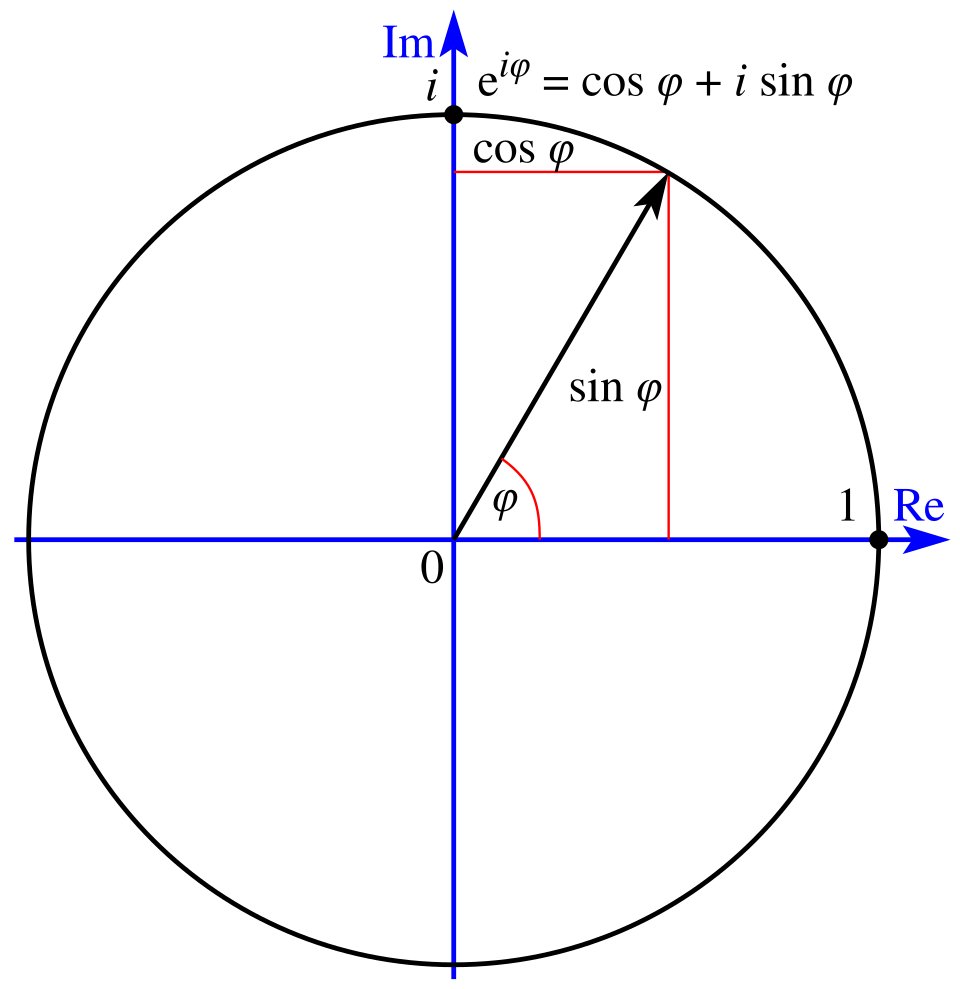
\includegraphics[
        width=0.55\textwidth
    ]{images/example_figure}

    \caption{Geometrical representation of sine and cosine on the
    unit circle.}

    \label{fig:unit_circle}
\end{figure}

When $\theta=\pi$, the corresponding point on the unit circle is
$(-1,0)$. Consequently, the imaginary component vanishes and Euler's
formula reduces to $e^{i\pi}=-1$.


% ============================================================
% EXAMPLE TABLE
% ============================================================

\section{The Constants in Euler's Identity}

One reason for the elegance of Euler's identity is the simultaneous
appearance of several fundamental mathematical constants
\cite{nahin2006euler}. Table~\ref{tab:constants} summarizes their
roles.

\begin{table}[htbp]

    \centering

    \caption{The fundamental constants appearing in Euler's identity.}

    \label{tab:constants}

    \begin{tabular}{cll}

        \toprule

        \textbf{Constant}
        & \textbf{Approximate value}
        & \textbf{Role} \\

        \midrule

        $0$
        & $0$
        & Additive identity \\

        $1$
        & $1$
        & Multiplicative identity \\

        $\pi$
        & $3.14159\ldots$
        & Circle constant \\

        $e$
        & $2.71828\ldots$
        & Base of the natural logarithm \\

        $i$
        & $\sqrt{-1}$
        & Imaginary unit \\

        \bottomrule

    \end{tabular}

\end{table}


% ============================================================
% DISCUSSION
% ============================================================

\section{The Elegance of the Identity}

The compactness of Euler's identity conceals connections among several
apparently different areas of mathematics. The constant $\pi$ arises
naturally from geometry, $e$ from analysis and exponential growth,
and $i$ from complex numbers.

Euler's formula brings these concepts together through trigonometric
functions and provides the bridge from the exponential function to
the geometry of the complex plane \cite{nahin2006euler}.

\subsection{A Compact Mathematical Relationship}

The equation is particularly striking because none of its five
constants is introduced artificially. Each has an independent and
fundamental role in mathematics, yet all five appear in the single
relation

\[
    e^{i\pi}+1=0.
\]

Its perceived elegance therefore comes not merely from its short
notation, but from the unexpectedly concise relationship it expresses
between otherwise distinct mathematical concepts.


% ============================================================
% CONCLUSIONS
% ============================================================

\section{Conclusions}

Euler's identity is a compact consequence of Euler's more general
formula for complex exponentials. Its connection with the unit circle
provides a simple geometrical interpretation, while the simultaneous
presence of $e$, $i$, $\pi$, $1$, and $0$ makes the identity an
especially elegant example of how different areas of mathematics can
be connected by a single equation.
% ============================================================
% END OF PAGES COUNTED TOWARD THE REPORT LIMIT
% ============================================================
%
% Everything before this point is part of the numbered report.
%
% For example, if the maximum report length is 25 pages,
% the final Conclusions page must not exceed page 25.
%
% References below are NOT included in the page count.
%
% ============================================================


\clearpage


% ============================================================
% REFERENCES
% ============================================================
%
% Disable page numbering so references are not included in the
% numbered report pages.
%

\pagenumbering{gobble}
\pagestyle{empty}

\printbibliography[
    heading=bibintoc,
    title={References}
]


\end{document}